%% LaTeX2e class for seminar theses
%% seminar.tex
%% 
%% Karlsruhe Institute of Technology
%% Institute for Program Structures and Data Organization
%% Chair for Software Design and Quality (SDQ)
%%
%% Dr.-Ing. Erik Burger
%% burger@kit.edu
%%
%% Version 1.0.1, 2018-04-16

%% Available page modes: oneside, twoside
%% Available languages: english, ngerman
%% Available modes: draft, final (see README)
\documentclass[twoside, english, draft]{Pflichtenheft}

%% ---------------------------------
%% | Information about the thesis  |
%% ---------------------------------

%% Name of the author
\author{PSE GRUPPE}

%% Title (and possibly subtitle) of the thesis
\title{Anomaly Detection in Industrial Networks}

%% Type of the thesis 
% \thesistype{Seminar Thesis}

%% Change the institute here, ``IPD'' is default
 \myinstitute{ KOMPETENZZENTRUM FÜR ANGEWANDTE SICHERHEITSTECHNOLOGIE }

%% The advisors are PhD Students or Postdocs
\advisor{M.Sc. Ankush Meshram}

\settitle

%% --------------------------------
%% | Settings for word separation |
%% --------------------------------

%% Describe separation hints here.
%% For more details, see 
%% http://en.wikibooks.org/wiki/LaTeX/Text_Formatting#Hyphenation
\hyphenation{
% me-ta-mo-del
}

%% --------------------------------
%% | Bibliography                 |
%% --------------------------------

%% Use biber instead of BibTeX, see README
\usepackage[citestyle=numeric,style=numeric,backend=biber]{biblatex}
\addbibresource{pflichtenheft.bib}

%% ====================================
%% ====================================
%% ||                                ||
%% || Beginning of the main document ||
%% ||                                ||
%% ====================================
%% ====================================
\begin{document}

%% Set PDF metadata
\setpdf

%% Set the title
\maketitle

%% ----------------
%% |   Abstract   |
%% ----------------
 This Document outlines the requirements (both functional and non-functional), environment, target audience, and use cases of the software described below.
%% The text is included from the following files:
%% - sections/abstract

%\begin{abstract}
%\%input{sections/abstract.tex}
%\end{abstract}

%% -----------------
%% |   Main part   |
%% -----------------

\thispagestyle{empty}
\newpage
\thispagestyle{empty}
\tableofcontents
\cleardoublepage
\setcounter{page}{1}


\section{Purpose}\label{sec:intro}
The goal of this project is to create a software visualization tool for industrial network traffic to simplify the analysis of anomalous behaviour, both in realtime and from captured stored data.
\\
This software is part of the ADIN framework and is referered to as the "ADIN Inspector".
\\
One component to achieve this goal is a web interface built with modularity in mind so as to make it easily extendable.
\\
The Web view is able to display a series of diagrams and charts to easily identify the behaviour of the network.
Within the Web view the user has the ability to zoom, select, highlight, and filter out data to better understand the aforementioned behaviour in different OSI layers, as well as visualize the flow rate between network nodes.
\\
To support this Web view a back-end messaging solution is needed. This allows the user to easily switch between multiple streams of captured data.
\\
\section{Overall Description}
\section{Interfaces}
\section{Functional Requirements}
\section{Data Requirements}
\section{Non-Functional Requirements}

\begin{itemize}
  \item{
  The web UI should be able to visualize the network topology and update the visualization based on real time data streams.
  }
  \item{
  The rendering latency should be no longer than 2 seconds.
  }
  \item{
  The framework should be able to handle data streamed from at least $\mathit{N}$ sensors.
  }
  \item{
  The framework should be able to save data collected in a specified period of time.
  }
  \item{
  The web UI should be viewable on modern web browsers.
  }
\end{itemize}

\section{Essential Testcases}
\section{Software Modelling}



\subsubsection{GUI}
The basic data structure needed for graphs are a given set of nodes and a given set of edges, as they are often drawn
as node-link diagrams. In the postal data set, nodes could represent the origins and destinations of postal flows. Edges represent the flows between the respective origins and destinations.In intelligence analysis, investigators use semantic graphs to organise concepts and relationships as
graph nodes and links in hopes of discovering key trends, patterns, and insights.”


A key issue in graph visualisation is the size of the graph, i.e. the size of the data to visualise. With a growing amount of data to display, graphs can become too complex and overburdening for the analyst’s cognitive capacity. It thus becomes difficult for the user to conduct significant analysis. Because of the issues described above, research often focuses on ways to solve the problems of visual clutter, e.g. by aggregation or clustering techniques, which is also one of the main topics of cartographic generalisation.

%%For example, Cui et al. (2008) investigate node-link diagrams for network visualisation.
%Their study focuses on the problem of visual cluttering in graph visualisations,
%as this is one of the main issues in the representation of relationships among
%large data (Herman, Melancon, and Marshall, 2000). They introduce a framework
%for geometry-based edge clustering to group edges into bundles and hence reduce
%visual cluttering caused by the crossing of the high number of edges (see figure 2.1).

\begin{figure}
\centering
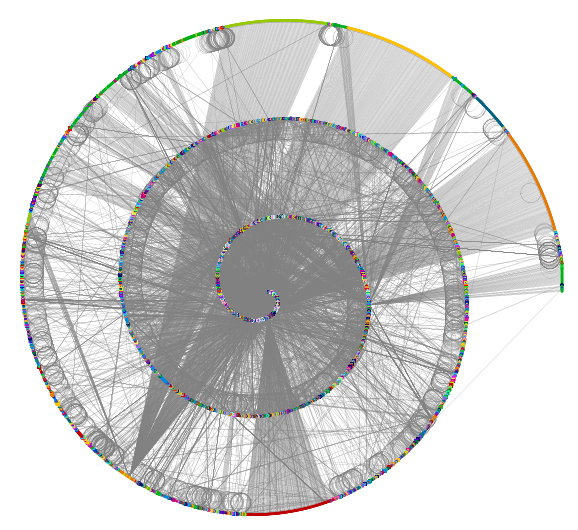
\includegraphics{node.jpg}
  \caption[ height=4cm, width=4cm]{Node-Link-Graph}
\end{figure}

\subsection{Scenario}

\begin{itemize}
\item{
/S100/ : An operator wants to check manually/visually whether network nodes appeared or disappeared over the last day
\begin{itemize}
\item{the operator opens the web page}
\item{the operator selects the database as data source}
\item{the operator selects a timeline-based display}
\item{the operator selects node addresses as the data to be displayed}
\item{the operator moves to or selects the last 24 hours as the range of data to display}
\item{the operator closes the web page}
  \end{itemize}
}


\item{
/S200/: A security analyst wants to look at the current flow rates between network nodes to see whether they change / there are trends
\begin{itemize}
\item{the analyst opens the web page}
\item{the analyst selects a source of live data}
\item{the analyst selects an appropriate visualization type}
\item{the analyst selects node adresses as the independent variable}
\item{the analyst selects flow rates as the data to be displayed}
\end{itemize}
}


\item{
/S300/: A security analyst wants to examine a specific point of data
\\
Precondition: the analyst has already selected the relevant dataset and visualization type
\begin{itemize}
\item{the analyst selects a data point by right-clicking}
\item{the GUI displays a small pop-up window with all the data of this data point}
\item{the analyst right-clicks one of the attibutes in the pop-up window and selects "Display all corresponding types"}
\item{the GUI marks all data points that have the same value in this attribute}
\end{itemize}
}


\item{
/S400/: The user wants to look at alarms/notifications
\begin{itemize}
\item{the user opens the web page}
\item{the user selects the database as data source}
\item{the user selects the data stream from the relevant dissector}
\item{the GUI diplays the notifications along a timeline, according to the time of the event}
\item{the user right-clicks on the x-axis and selects "use record number"}
\item{the GUI diplays the notifications along a timeline adjacently}
\end{itemize}
}


\item{
/S500/: The user wants to look at normal data together with alarms/notifications
\\
Precondition: Scenario /S100/ apart from closing the web page
\begin{itemize}
\item{the user selects menu "data", entry "sources"}
\item{the GUI displays a list of all known data sources with a checkbox in front of each}
\item{the user selects the checkboxes for the data sources they want to examine}
\item{the GUI displays data from all these data sources within the currently active visualization}
\end{itemize}
}

\end{itemize}

\subsection{Use cases}
\subsubsection{Interactivity}


Visual analytics methods combine interactive visualisations with automated analysis
techniques. This allows the user to decide e.g. which part
of the data he or she wants to explore in more detail.

 A basic principle for visual data exploration was introduced by Shneiderman (1997) by what he called the “The
Visual Information Seeking Mantra: 

Overview first, zoom and filter, then details-ondemand”.
This lets the data analyst define to a certain level what he or she wants
to see and visualise. 

Similar to this, Bertin (1983) specified three “levels of reading,”:
The elementary level (allowing the analyst to look at the information about a
single data record), the intermediate level (showing summarised information about a group of data records), and the global level (providing an overview of all data elements).

\subsection{Object Modelling}
\subsection{Dynamic Modelling}
\subsection{User Interface}
\subsection{Glossary}

%% |   Bibliography   |
%% --------------------

%% Add entry to the table of contents for the bibliography
\printbibliography[heading=bibintoc]

\end{document}
